% !Mode:: "TeX:UTF-8"
% !TEX program  = xelatex



\documentclass{hfutreport}
%\documentclass[bwprint]{hfutreport} %打印的时候有超链接的地方不需要彩色,可以加上bwprint 选项

\usepackage{fontspec}
\usepackage{listings}
\usepackage{upquote}
\usepackage{graphicx}
\usepackage{xcolor} % Custom color definitions

% Color definitions
\definecolor{lightgray}{rgb}{0.95, 0.95, 0.95}
\definecolor{darkgray}{rgb}{0.4, 0.4, 0.4}
%\definecolor{purple}{rgb}{0.65, 0.12, 0.82}
\definecolor{editorGray}{rgb}{0.95, 0.95, 0.95}
\definecolor{editorOcher}{rgb}{1, 0.5, 0} % #FF7F00 -> rgb(239, 169, 0)
\definecolor{editorGreen}{rgb}{0, 0.5, 0} % #007C00 -> rgb(0, 124, 0)
\definecolor{orange}{rgb}{1,0.45,0.13}		
\definecolor{olive}{rgb}{0.17,0.59,0.20}
\definecolor{brown}{rgb}{0.69,0.31,0.31}
\definecolor{purple}{rgb}{0.38,0.18,0.81}
\definecolor{lightblue}{rgb}{0.1,0.57,0.7}
\definecolor{lightred}{rgb}{1,0.4,0.5}
\definecolor{str_color}{RGB}{106,135,89}
\definecolor{background_color}{RGB}{43,43,43}
\definecolor{key_color}{RGB}{204,120,50}
\definecolor{comment_color}{RGB}{128,128,128}

% CSS
\lstdefinelanguage{css}{
  keywords={color,background-image:,margin,padding,font,weight,display,position,top,left,right,bottom,list,style,border,size,white,space,min,width, transition:, transform:, transition-property, transition-duration, transition-timing-function},	
  sensitive=true,
  morecomment=[l]{//},
  morecomment=[s]{/*}{*/},
  morestring=[b]',
  morestring=[b]",
  alsoletter={:},
  alsodigit={-}
}

% JavaScript
\lstdefinelanguage{javascript}{
  morekeywords={typeof, new, true, false, catch, function, return, null, catch, switch, var, if, in, while, do, else, case, break},
  morecomment=[s]{/*}{*/},
  morecomment=[l]//,
  morestring=[b]",
  morestring=[b]'
}

\lstdefinelanguage{html5}{
  language=html,
  sensitive=true,	
  alsoletter={<>=-},	
  morecomment=[s]{<!-}{-->},
  tag=[s],
  otherkeywords={
  % General
  >,
  % Standard tags
	<!DOCTYPE,
  </html, <html, <head, <title, </title, <style, </style, <link, </head, <meta, />,
	% body
	</body, <body,
	% Divs
	</div, <div, </div>, 
	% Paragraphs
	</p, <p, </p>,
	% scripts
	</script, <script,
  % More tags...
  <canvas, /canvas>, <svg, <rect, <animateTransform, </rect>, </svg>, <video, <source, <iframe, </iframe>, </video>, <image, </image>, <header, </header, <article, </article
  },
  ndkeywords={
  % General
  =,
  % HTML attributes
  charset=, src=, id=, width=, height=, style=, type=, rel=, href=,
  % SVG attributes
  fill=, attributeName=, begin=, dur=, from=, to=, poster=, controls=, x=, y=, repeatCount=, xlink:href=,
  % properties
  margin:, padding:, background-image:, border:, top:, left:, position:, width:, height:, margin-top:, margin-bottom:, font-size:, line-height:,
	% CSS3 properties
  transform:, -moz-transform:, -webkit-transform:,
  animation:, -webkit-animation:,
  transition:,  transition-duration:, transition-property:, transition-timing-function:,
  }
}

% lstset configuration for code style
\lstset{
    basicstyle=\small\color{white}, % Set basic font and color
    numbers=left, % Line numbers on the left
    numberstyle=\tiny\color{white}, % Line number style
    breaklines=true, % Automatic line breaking
    backgroundcolor=\color{background_color}, % Background color
    keywordstyle=\color{key_color}, % Keyword color
    stringstyle=\color{str_color}, % String literal color
    commentstyle=\color{comment_color}, % Comment color
    frame=single, % Single frame around the code
    tabsize=4, % Tab size
    showspaces=false, % Do not show spaces
}

\title{软件开发实训}
\stunum{2021211629}
\stuname{万嘉豪}
\stuclass{数学与应用数学21-2班}
\supervisor{王琦}
\dateinput{\today}
\maincontent{编写了一个一般性的静态网页,可以自定义倒计时,番茄钟,设置背景图,主题切换等。网页主体分为三个大类,左上为倒计时板块,右上为番茄钟板块,最下方是一言 API。使用方法为直接在浏览器打开即可。如果第一次打开网页时没有显示内容,请先设置深色背景图,在文件夹有一张默认背景图,请复制名称输入即可(包含扩展名);默认目标倒计时 为 2024-12-23;番茄钟的作息为 25-5-25-5-15 循环。}

\begin{document}

 \maketitle

% 设置钻字体

\setmainfont{MesloLGS NF Regular}

% 目录使用Romen页脚 
\pagestyle{plain}
\pagenumbering{Roman}
\tableofcontents
\newpage
\pagestyle{plain}

%正文页脚
\setcounter{page}{1}
\pagenumbering{arabic}

\section{初心}
最近在准备考研,正好老师说这个课程设计可以自由发挥,晚上洗澡的时候就想好功能了:能够提醒我距离考试还有多少天,以及安排我的学习休息时间。

\section{开发过程}

我开始想的比较简单,就上面两个功能所以很快就写好了。

\subsection{ 一言 API}

\begin{lstlisting}[language=javascript]
function fetchHitokoto() {
  fetch('https://v1.hitokoto.cn')
    .then(response => response.json())
    .then(data => {
      document.getElementById('hitokoto').innerText = data.hitokoto + " —— " + data.from;
    })
    .catch(console.error);
}
\end{lstlisting}

\subsection{目标倒计时}

此处的目标倒计时定死了倒计时的日期,虽然也满足了需求,但是缺少了其他应用的可能性,会在下面的部分打上补丁,设置自定义目标日期。

\begin{lstlisting}[language=javascript]
function updateExamCountdown() {
  const examDate = new Date('2024-12-23');
  const currentDate = new Date();
  const timeDiff = examDate - currentDate;
  const days = Math.ceil(timeDiff / (1000 * 60 * 60 * 24));
  document.getElementById('examCountdown').innerText = `距离考研还有 ${days} 天`;
}
\end{lstlisting}


\subsection{番茄钟}

普通的番茄钟只能简单的计时然后休息,但是长时间的短休息不能让身体得到充分的放松,我加入了长短休息交替的判断逻辑,能够在进行两次 25-5 循坏后切换 -15 的长休息时间。

\begin{lstlisting}[language=javascript]
let pomodoroTimer = null;
let isWorkTime = true;
let timeLeft = 25 * 60;

function startPomodoro() {
  if (!pomodoroTimer) {
    pomodoroTimer = setInterval(updatePomodoro, 1000);
  }
}

function pausePomodoro() {
  clearInterval(pomodoroTimer);
  pomodoroTimer = null;
}

function updatePomodoro() {
  if (timeLeft <= 0) {
    if (isWorkTime) {
      workSessions++;
      isWorkTime = false;
      timeLeft = (workSessions % 4 === 0) ? 15 * 60 : 5 * 60;
      alert('工作结束,开始休息!');
    } else {
      isWorkTime = true;
      timeLeft = 25 * 60;
      alert('休息结束,开始工作!');
    }
  } else {
    timeLeft--;
    document.getElementById('pomodoro').innerText = isWorkTime ? `工作时间: ${Math.floor(timeLeft / 60)}:${(timeLeft % 60).toString().padStart(2, '0')}` : `休息时间: ${Math.floor(timeLeft / 60)}:${(timeLeft % 60).toString().padStart(2, '0')}`;
  }
}
\end{lstlisting}

\subsection{更改背景图}

在背景图的设置中,我加入了 local storage 的储存方式,让浏览器缓存背景图 URL,这样就可以通过替换 URL 得到完全不同的背景,加强了用户体验。在第一次打开静态网页时,需要先在网页目录'./'中添加一张图片,然后复制名称提交到网页,不然最开始设置的背景是看不清楚网页的。例如'./64ddee7f78086b60daa38b51.jpg',请保留文件的扩展名。

\begin{lstlisting}[language=javascript]
function setBackgroundImage() {
  const imageUrl = prompt("请输入新的背景图片URL:");
  if (imageUrl) {
    document.body.style.backgroundImage = `url('${imageUrl}')`;
    localStorage.setItem('backgroundImage', imageUrl);
  }
}

function loadBackgroundImage() {
  const imageUrl = localStorage.getItem('backgroundImage');
  if (imageUrl) {
    document.body.style.backgroundImage = `url('${imageUrl}')`;
  }
}
\end{lstlisting}


\section{老师的建议}
王琦老师给我提出了宝贵的建议:让倒计时可以自定义,使其变得更有普适性;同时希望我能加入一点其他功能,让页面看起来更舒服一点。于是我更改了目标倒计时的代码,同时加入了心的主题设置的功能。

\begin{lstlisting}[language=javascript]
function setCustomCountdown() {
  const customDate = prompt("默认考研日期,请输入倒计时的目标日期 (格式: YYYY-MM-DD):");
  if (customDate) {
    localStorage.setItem('customCountdownDate', customDate);
    updateExamCountdown();
  }
}

function updateExamCountdown() {
  let countdownDate = localStorage.getItem('customCountdownDate');
  if (!countdownDate) {
    countdownDate = '2024-12-23'; // 默认考研日期
  }
  const targetDate = new Date(countdownDate);
  const currentDate = new Date();
  const timeDiff = targetDate - currentDate;
  const days = Math.ceil(timeDiff / (1000 * 60 * 60 * 24));
  document.getElementById('examCountdown').innerText = `距离目标日期还有 ${days} 天`;
}

function changeTheme(themeName) {
  document.body.className = themeName + '-theme';
  localStorage.setItem('selectedTheme', themeName);
}

function loadTheme() {
  const selectedTheme = localStorage.getItem('selectedTheme') || 'default';
  changeTheme(selectedTheme);
  document.getElementById('themeSelector').value = selectedTheme;
}

window.onload = function() {
  loadBackgroundImage();
  loadTheme();
  fetchHitokoto();
  updateExamCountdown();
};
\end{lstlisting}

\newpage
\section{成品}

\begin{figure}[hbtp]
  \centering
  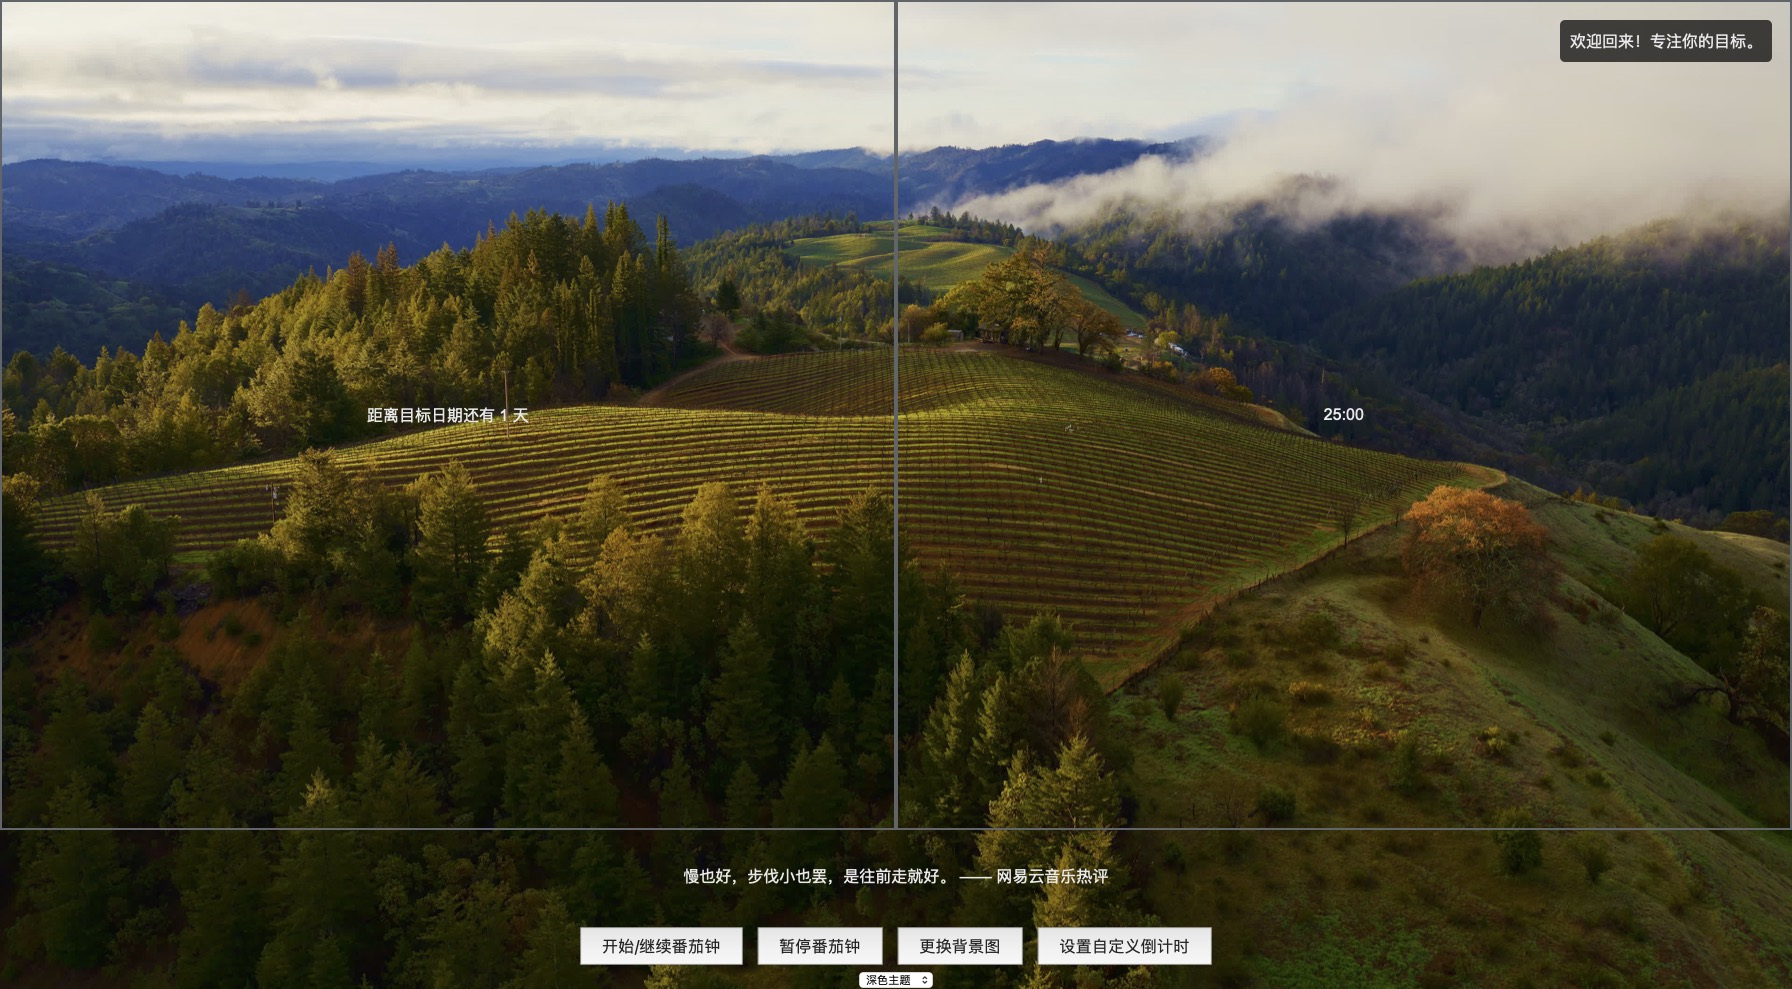
\includegraphics[scale=0.25]{/Users/xnhxjx/Desktop/HFUT_Course_Report_Template.V1.1/figures/最终版本.pdf}
  \caption{最终版本}
\end{figure}


%附录
\begin{appendices}
\section{源代码——格式部分}

\begin{lstlisting}[language=html5]
<style>
  /* 默认主题 */
  :root {
    --bg-color: #282c34;
    --text-color: #fff;
    --border-color: #fff;
  }

  /* 深色主题 */
  .dark-theme {
    --bg-color: #1c2025;
    --text-color: #eaeaea;
    --border-color: #606468;
  }

  /* 浅色主题 */
  .light-theme {
    --bg-color: #f0f0f0;
    --text-color: #333;
    --border-color: #ddd;
  }

  body {
    font-family: Arial, sans-serif;
    background-size: cover;
    color: var(--text-color);
    background-color: var(--bg-color);
    display: flex;
    flex-direction: column;
    align-items: center;
    height: 100vh;
    margin: 0;
    overflow: hidden;
  }
  .main-content {
    display: flex;
    width: 100%;
    height: 90%;
  }
  .block {
    flex: 1;
    display: flex;
    justify-content: center;
    align-items: center;
    text-align: center;
    border: 2px solid var(--border-color);
    padding: 20px;
  }
  #hitokoto {
    width: 100%;
    text-align: center;
    height: 10%;
    display: flex;
    justify-content: center;
    align-items: center;
  }
  button {
    margin: 5px;
    padding: 10px 20px;
    font-size: 16px;
  }
  .tooltip {
    position: fixed;
    top: 20px;
    right: 20px;
    background-color: rgba(0, 0, 0, 0.7);
    color: var(--text-color);
    padding: 10px;
    border-radius: 5px;
  }
</style>

\end{lstlisting}

\section{源代码——主体部分}

\begin{lstlisting}[language=html5]
<div class="tooltip">欢迎回来!专注你的目标。</div>
<div class="main-content">
  <div id="examCountdown" class="block">倒计时加载中...</div>
  <div id="pomodoro" class="block">25:00</div>
</div>
<div id="hitokoto">一言加载中...</div>
<div>
  <button onclick="startPomodoro();">开始/继续番茄钟</button>
  <button onclick="pausePomodoro();">暂停番茄钟</button>
  <button onclick="setBackgroundImage();">更换背景图</button>
  <button onclick="setCustomCountdown();">设置自定义倒计时</button>
</div>
<div>
  <select id="themeSelector" onchange="changeTheme(this.value);">
    <option value="default">默认主题</option>
    <option value="dark">深色主题</option>
    <option value="light">浅色主题</option>
  </select>
</div>

\end{lstlisting}

\section{源代码——脚本部分}

\begin{lstlisting}[language=javascript]
let workSessions = 0;

function fetchHitokoto() {
  fetch('https://v1.hitokoto.cn')
    .then(response => response.json())
    .then(data => {
      document.getElementById('hitokoto').innerText = data.hitokoto + " —— " + data.from;
    })
    .catch(console.error);
}

function setCustomCountdown() {
  const customDate = prompt("默认考研日期,请输入倒计时的目标日期 (格式: YYYY-MM-DD):");
  if (customDate) {
    localStorage.setItem('customCountdownDate', customDate);
    updateExamCountdown();
  }
}

function updateExamCountdown() {
  let countdownDate = localStorage.getItem('customCountdownDate');
  if (!countdownDate) {
    countdownDate = '2024-12-23'; // 默认考研日期
  }
  const targetDate = new Date(countdownDate);
  const currentDate = new Date();
  const timeDiff = targetDate - currentDate;
  const days = Math.ceil(timeDiff / (1000 * 60 * 60 * 24));
  document.getElementById('examCountdown').innerText = `距离目标日期还有 ${days} 天`;
}

let pomodoroTimer = null;
let isWorkTime = true;
let timeLeft = 25 * 60;

function startPomodoro() {
  if (!pomodoroTimer) {
    pomodoroTimer = setInterval(updatePomodoro, 1000);
  }
}

function pausePomodoro() {
  clearInterval(pomodoroTimer);
  pomodoroTimer = null;
}

function updatePomodoro() {
  if (timeLeft <= 0) {
    if (isWorkTime) {
      workSessions++;
      isWorkTime = false;
      timeLeft = (workSessions % 4 === 0) ? 15 * 60 : 5 * 60;
      alert('工作结束,开始休息!');
    } else {
      isWorkTime = true;
      timeLeft = 25 * 60;
      alert('休息结束,开始工作!');
    }
  } else {
    timeLeft--;
    document.getElementById('pomodoro').innerText = isWorkTime ? `工作时间: ${Math.floor(timeLeft / 60)}:${(timeLeft % 60).toString().padStart(2, '0')}` : `休息时间: ${Math.floor(timeLeft / 60)}:${(timeLeft % 60).toString().padStart(2, '0')}`;
  }
}

function setBackgroundImage() {
  const imageUrl = prompt("请输入新的背景图片URL:");
  if (imageUrl) {
    document.body.style.backgroundImage = `url('${imageUrl}')`;
    localStorage.setItem('backgroundImage', imageUrl);
  }
}

function loadBackgroundImage() {
  const imageUrl = localStorage.getItem('backgroundImage');
  if (imageUrl) {
    document.body.style.backgroundImage = `url('${imageUrl}')`;
  }
}

function changeTheme(themeName) {
  document.body.className = themeName + '-theme';
  localStorage.setItem('selectedTheme', themeName);
}

function loadTheme() {
  const selectedTheme = localStorage.getItem('selectedTheme') || 'default';
  changeTheme(selectedTheme);
  document.getElementById('themeSelector').value = selectedTheme;
}

window.onload = function() {
  loadBackgroundImage();
  loadTheme();
  fetchHitokoto();
  updateExamCountdown();
};
</script>

\end{lstlisting}

\end{appendices}

\end{document} 